%%% TeX-command-extra-options: "-shell-escape"
\documentclass[11pt]{article}

\usepackage{latexsym}
\usepackage{amsmath}
\usepackage{amssymb}
\usepackage{amsthm}
\usepackage{graphicx}
\usepackage{wrapfig}
\usepackage{pseudocode}
\usepackage{url}
\usepackage[backref, colorlinks=true, citecolor=red, urlcolor=blue, pdfauthor={Jyh-Ming Lien}]{hyperref}
\usepackage{svg}
\usepackage{float}


\newcommand{\handout}[5]{
  \noindent
  \begin{center}
    \framebox{
      \vbox{
        \hbox to 5.78in { {\bf } \hfill #2 }
        \vspace{4mm}
        \hbox to 5.78in { {\Large \hfill #5  \hfill} }
        \vspace{2mm}
        \hbox to 5.78in { {\em #3 \hfill #4} }
      }
    }
  \end{center}
  \vspace*{4mm}
}

\newcommand{\lecture}[4]{\handout{#1}{#2}{#3}{#4}{#1}}

\newtheorem{theorem}{Theorem}
\newtheorem{corollary}[theorem]{Corollary}
\newtheorem{lemma}[theorem]{Lemma}
\newtheorem{observation}[theorem]{Observation}
\newtheorem{proposition}[theorem]{Proposition}
\newtheorem{definition}[theorem]{Definition}
\newtheorem{claim}[theorem]{Claim}
\newtheorem{fact}[theorem]{Fact}
\newtheorem{assumption}[theorem]{Assumption}

% 1-inch margins, from fullpage.sty by H.Partl, Version 2, Dec. 15, 1988.
\topmargin 0pt
\advance \topmargin by -\headheight
\advance \topmargin by -\headsep
\textheight 8.9in
\oddsidemargin 0pt
\evensidemargin \oddsidemargin
\marginparwidth 0.5in
\textwidth 6.5in

\parindent 0in
\parskip 1.5ex
% \renewcommand{\baselinestretch}{1.25}

\begin{document}

\lecture{Hedcuter Assignment}{Fall 2017}{Bryan Hoyle}{Computational Geometry}

\section{Summary of the two methods}

\subsection{hedcuter method}

This method uses the wavefront method to compute voronoi cells. First,
it oversizes the image in order to do subpixel sampling. Next, it
actually computes to which cell point to which each subpixel
belongs. To do this, it maintains a weighted queue of points keyed by
weighted distance from front (and if the weighted distances are the
same, it chooses priority based on the the horizontal posistions, and
if those are the same, the vertical positions). It then checks the
current subpixel it is on to see if any of its neighbors could belong
to a closer voronoi cell. If so, they are updated and the wavefront is
updated to contain the changed subpixel. Once it is done with all of
the wavefronts, it then does a reverse lookup for every pixel to add
it to the cell's ownership list. It then computes the weighted
centroid using the density function described
in~\cite{stippling}. Afterwards, it moves the center of each cell to
the respective centroid. It repeats this process until either the
desired number of iterations is reached or the displacement reached
some minimum. It then renders the stipples using average color of the
cell in RGB space and the radius is either uniform to what was set or,
if varying disk size is allowed, it's set to be scaled by the average
value of cell's color.

\subsection{voronoi method}

The voronoi method is rather easy. It iterates a weighted relaxation
based on the density function described in the paper. To compute the
voronoi diagram, it uses Fortune's algorithm. When it's computing the
centroid, it computes the clip lines of the cell and grabs a ``tile''
by using the bounding box of the cell. It then scales the tile to the
desired size (for use in subsampling). Then, it iterates over every
pixel in the tile and uses the clip lines to determine if the pixel is
in the cell. If it is in the cell, it updates both the weight of the
cell and the maximum possible weight of the cell by using the
intensity of the pixel. Then, it computes the radius of the stipple
(if it is set to bound by the cell, it uses the biggest possible
internal radius of the cell, otherwise, it uses the biggest possible
radius that has an edge intersecting the stipple). It uses the ratio
of the weight to the maximum possible weight to scale the radius of
the stipple (the darker the image in the voronoi cell, the larger the
radius). It then sets the center of the cell to the weighted
centroid. It repeats the loop of computing the voronoi diagram then
using weighted relaxation until the average displacement of the
relaxation is very small (meaning that it didn't change much). When it
is done, it just renders the diagram by sampling the cell point for
color (if color mode is enabled, otherwise, it uses a black circle)
and then rendering the stipples as circles of the computed radius.

\section{Comparison of the two methods}

\subsection{Do you get the same results by running the same program on the same image multiple times?}

The voronoi\_stippler program does give the same results each time,
however, the hedcuter executable does not. This is because the the
voronoi\_stippler code uses the same seed each time it is run for the
random number generator. The hedcuter code does not use the same seed
each time.

\begin{figure}[H]
  \centering
  \begin{minipage}{.5\textwidth}
    \centering
    \includesvg[width=0.95\textwidth]{A1}
  \end{minipage}%
  \begin{minipage}{.5\textwidth}
    \centering
    \includesvg[width=0.95\textwidth]{A2}
  \end{minipage}
  \caption{Comparison of two runs of hedcuter on the same image using
    the same parameters. Notice the hair (circled in red) is different}
\end{figure}

\subsection{If you vary the number of the disks in the output images,
  do these implementations produce the same distribution in the final
  image? If not, why?}

It seems like the hedcuter implementation crowds the dark areas more
heavily (which makes sense, as it uses the darkness of a pixel when
calculating the voronoi diagram as part of the distance). Also, the
voronoi\_stippler seems more uniform in its final output.  See
figures~\ref{hc_b} and~\ref{vs_b} for comparison of output.

\begin{figure}[h]
  \centering
  \begin{minipage}{.32\textwidth}
    \centering
    \includesvg[width=0.95\textwidth]{B1}
  \end{minipage}%
  \begin{minipage}{.32\textwidth}
    \centering
    \includesvg[width=0.95\textwidth]{B2}
  \end{minipage}
  \begin{minipage}{.32\textwidth}
    \centering
    \includesvg[width=0.95\textwidth]{B3}
  \end{minipage}
  \caption{Three runs of 100, 1000, and 10000 disks using the hedcuter
  program. Notice that it crowds more heavily towards black areas.}\label{hc_b}
\end{figure}

\begin{figure}[H]
  \centering
  \begin{minipage}{.32\textwidth}
    \centering
    \includesvg[width=0.95\textwidth]{B4}
  \end{minipage}%
  \begin{minipage}{.32\textwidth}
    \centering
    \includesvg[width=0.95\textwidth]{B5}
  \end{minipage}
  \begin{minipage}{.32\textwidth}
    \centering
    \includesvg[width=0.95\textwidth]{B6}
  \end{minipage}
  \caption{Three runs of 100, 1000, and 10000 disks using the
    voronoi\_stippler program. This output is more uniform across the
    image.}\label{vs_b}
\end{figure}

\subsection{If you vary the number of the disks in the output images,
  is a method faster than the other?}

Yes. The voronoi\_stippler method actually speeds up with more
disks. Hedcuter gets slower the more disks were added. For example,
for figure~\ref{hc_b}, the times to compute were 32, 38, and 43
seconds respectively, however, for figure~\ref{vs_b}, the times to
compute were 54, 46, and 7 seconds, respectively.

\subsection{Does the type of image increase or descrease their difference?}

Because the hedcuter method is more heavily weighted towards the dark
areas, cartoon drawings like the klaymen image are very different than
the voronoi\_stippler method. Because of the fact that hedcuter uses
darkness as a part of its cell calculation step, you can also see that
it concentrates more heavily along edges between colors, thus images
with high contrast or lots of sudden value changes will have more
focus on the edges than the voronoi\_stippler method. See
figures~\ref{c1} and~\ref{c2} for examples of strongly edged images,
and~\ref{c3} for a human portrait.

\begin{figure}[H]
  \centering
  \begin{minipage}{.5\textwidth}
    \centering
    \includesvg[width=0.95\textwidth]{C1}
  \end{minipage}%
  \begin{minipage}{.5\textwidth}
    \centering
    \includesvg[width=0.95\textwidth]{C2}
  \end{minipage}
  \caption{Hedcuter (left) vs voronoi\_stippler (right) for a cartoon
    image. Note the concentration of stipples along the edges of the
    character and the background circle for the hedcut
    implementation.}\label{c1}
\end{figure}

\begin{figure}[H]
  \centering
  \begin{minipage}{.5\textwidth}
    \centering
    \includesvg[width=0.95\textwidth]{C3}
  \end{minipage}%
  \begin{minipage}{.5\textwidth}
    \centering
    \includesvg[width=0.95\textwidth]{C4}
  \end{minipage}
  \caption{Hedcuter (left) vs voronoi\_stippler (right) for another cartoon image.}\label{c2}
\end{figure}

\begin{figure}[H]
  \centering
  \begin{minipage}{.5\textwidth}
    \centering
    \includesvg[width=0.95\textwidth]{C5}
  \end{minipage}%
  \begin{minipage}{.5\textwidth}
    \centering
    \includesvg[width=0.95\textwidth]{C6}
  \end{minipage}
  \caption{Hedcuter (left) vs voronoi\_stippler (right) for a
    portrait. Note that I turned up the radius of the hedcuter disks
    for this example so that one can better see the pattern
    differences. Highlighted is an area where the hedcuter program
    spent more cells in the fine detail.}\label{c3}
\end{figure}

\subsection{Are the outputs of these stippling methods different than
  the hedcut images created by artists (e.g.\ those from the Wall
  Street Journal)?}

Very different. Figure~\ref{faces} shows an artist created hedcut
image. Notice that instead of using just the darkness of a reference
image for density stippling, it uses the countours of a 3d
surface. This meta-information is not easily available to a program
running on a photo, but, it creates much more natural looking images.

\begin{figure}[H]
  \centering
  \begin{minipage}{1\textwidth}
    \centering
    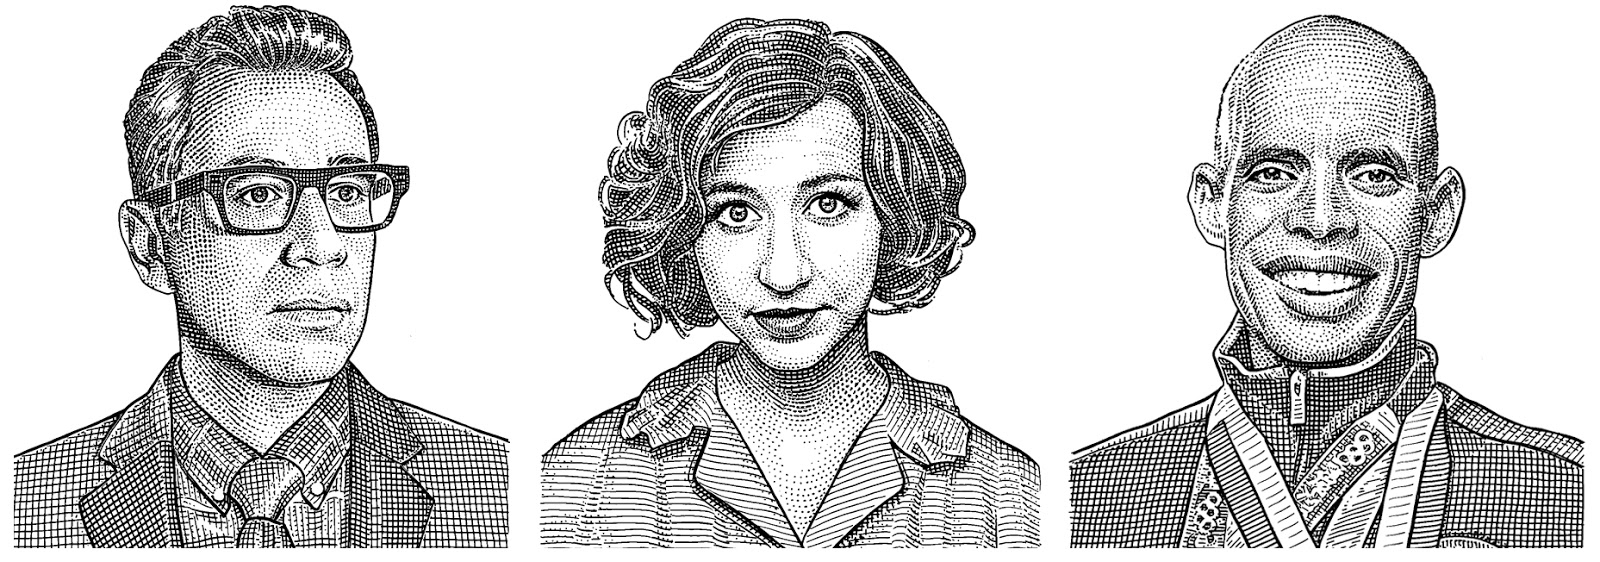
\includegraphics[width=0.95\textwidth]{faces.jpg}
  \end{minipage}
  \caption{Artist created stipple portraits. Retrieved
    from~\cite{facesimg}}\label{faces}
\end{figure}


\section{Improvement of hedcuter method}
\subsection{Use a percepual color space}
The first thing I did was to use a perceptual color space (CIELab with
illuminant D65) in order to get distance from white. And used that
instead of the default value usage. This did not provide much visual
improvement on its own other than reducing some of the unnatural
clustering of points near edges, but came in handy for the next two
improvements. Note that you can zoom in on the pdf to see the images
better as I included the svgs directly.  \nocite{tree}

\begin{figure}[H]
  \centering
  \begin{minipage}{.5\textwidth}
    \centering
    \includesvg[width=0.95\textwidth]{D1}
  \end{minipage}%
  \begin{minipage}{.5\textwidth}
    \centering
    \includesvg[width=0.95\textwidth]{D2}
  \end{minipage}
  \caption{Left is before perceptual weighting, right is after. Note
    that the images look basically the same, with a little less
    unnatural clustering near the edges of objects.}
\end{figure}

\subsection{Use a variable background color}
The next thing I did is allowed an image to specify a different
background color than white. It takes this into account for the
density function and creates a more optimal stipple for the chosen
background color. The disk size is now based on the average distance
from the background color. 

\begin{figure}[H]
  \centering
  \begin{minipage}{.5\textwidth}
    \centering
    \includesvg[width=0.95\textwidth]{D2}
  \end{minipage}%
  \begin{minipage}{.5\textwidth}
    \centering
    \includesvg[width=0.95\textwidth]{E2}
  \end{minipage}
  \caption{Variable colored backgrounds}
\end{figure}

\subsection{Better Disk Rendering}
I liked the output scaling of the disks in the bounded by cell size in
voronoi\_stippler better, so I replicated that in hedcuter. This
creates much more balanced images, in my opinion.

\begin{figure}[H]
  \centering
  \begin{minipage}{.5\textwidth}
    \centering
    \includesvg[width=0.95\textwidth]{E2}
  \end{minipage}%
  \begin{minipage}{.5\textwidth}
    \centering
    \includesvg[width=0.95\textwidth]{F1}
  \end{minipage}
  \caption{Default on the left, new scaling on the right. Note how the
    image has better scaling of the stipples}
\end{figure}



\bibliographystyle{plain}
\bibliography{report}

\end{document}


